\section{TF-IDF}\label{sec:tfidf}

\subsection{¿Qué es el TF-IDF?}
\begin{frame}{¿Qué es el TF-IDF?}
    \begin{center}
        Tf-idf (del inglés Term frequency - Inverse document frequency), frecuencia de término - 
        frecuencia inversa de documento (o sea, la frecuencia de ocurrencia del término en la colección de documentos),
        es una medida numérica que expresa cuán relevante es una palabra para un documento en una colección.\\
        \pause
        \vspace*{1cm}
        El valor tf-idf aumenta proporcionalmente al número de veces que una palabra aparece en el documento, 
        pero es compensada por la frecuencia de la palabra en la colección de documentos, lo que permite 
        manejar el hecho de que algunas palabras son generalmente más comunes que otras.
    \end{center}
\end{frame}

\begin{frame}{¿Qué es el TF-IDF?}
    \begin{figure}
        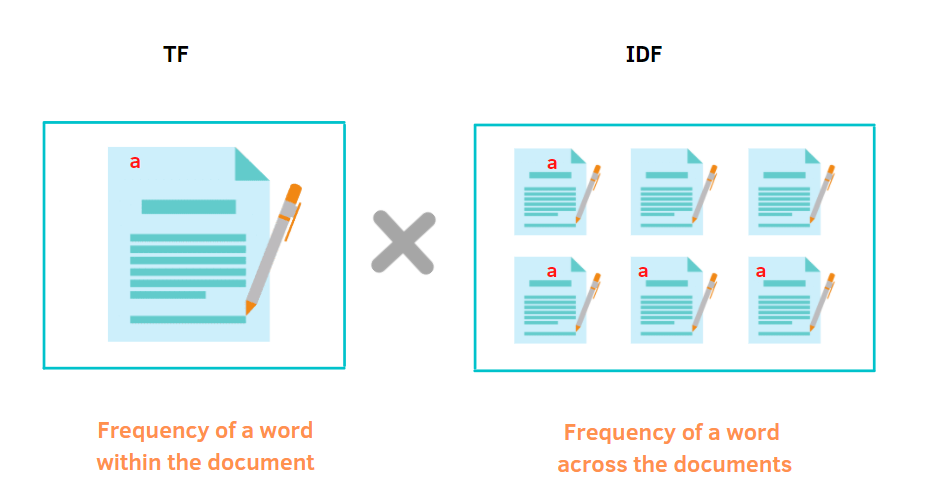
\includegraphics[width=0.9\framewidth]{fotos/tfidf.png}
    \end{figure}
\end{frame}

\subsection{Ecuacion del TF-IDF}
\begin{frame}{Ecuacion del TF-IDF}
    El TF-IDF se calcula a través de la siguientes formulas:
    \begin{equation}
        tf(t,d) = \frac{f(t,d)}{max(f(d))}
    \end{equation}

    \begin{equation}
        idf(t,D) = \log\frac{D}{D(t)}
    \end{equation}

    \begin{equation}
        tfidf(t,d,D) = tf(t,d) \cdot idf(t.D)
    \end{equation}

    donde:
    \begin{itemize}
        \item f (t,d): frecuencia de la palabra t en el documento d 
        \item max(f(d)): máxima frecuencia de una palabra en el documento d
        \item D: número de documentos de la colección 
        \item D(t): número de documentos donde aparece la palabra t
    \end{itemize}
\end{frame}

\subsection{Matriz de TF-IDF}
\begin{frame}{Matriz de TF-IDF}
    \begin{center}
        Y una vez que se haya calculado los tf-idf de las palabras de todos los documentos, estos van a ser guardados
        en una matriz, en donde las columnas seran las palabras y las filas los documentos.

        \vspace*{1.5cm}

        En este proyecto, la clase \textit{Terms} es la encargada de realizar toda la implentación del TF-IDF
    \end{center}
\end{frame}